% Created 2021-04-28 mer. 10:16
% Intended LaTeX compiler: pdflatex
\documentclass[presentation]{beamer}
\usepackage[orientation=portrait,size=a0,scale=1.4,debug]{beamerposter}
\usepackage[overlay]{textpos}
\usepackage[utf8]{inputenc}
\usepackage[T1]{fontenc}
\usepackage{graphicx}

\newtheorem{assumption}{Assumption}%[numberby]
\newtheorem{remark}{Remark}%[numberby]
\usepackage[ruled,noend,algo2e]{algorithm2e}
\usepackage{fontawesome}
\usepackage{pgfplots}
\usepackage{grffile}
\usepackage{longtable}
\usepackage{wrapfig}
\usepackage{rotating}
\usepackage[normalem]{ulem}
\usepackage{amsmath}
\usepackage{textcomp}
\usepackage{amssymb}
\usepackage{booktabs}
\usepackage{capt-of}
\usepackage{hyperref}
\usepackage{tikz}
\usepackage{circuitikz}
\usetikzlibrary{arrows.meta,calc}
\usetikzlibrary{calc,shapes,positioning}

% \usepackage[french]{babel}
\usepackage[english]{babel}
\usepackage{amsmath}
\usepackage{graphicx}
\usepackage[utf8]{inputenc}
\usepackage{pgfpages}
\usepackage{multicol}
\usepackage{totcount}
\regtotcounter{section}

\usepackage{amsmath}
\usepackage{mathtools}
\usepackage{amssymb}
\usepackage{picture}
\usepackage{bbding}
\usepackage{bbold}
\usepackage{sansmathaccent}
\pdfmapfile{+Sensationsmache.map}
\usepackage{stmaryrd}
\usepackage{tikz}

% \newcommand\warning[1]{\ifdebug {\color{red}#1}\fi}

\usepackage{hyperref}
\usepackage{natbib}
\usepackage{cancel}
\usepackage{ulem}

\usetheme{default}
\author{Rafael Accácio Nogueira, Romain Bourdais, Simon Leglaive, Hervé Guéguen}


\date{\today}
\title{Expectation-Maximization based defense mechanism for dMPC}
\institute{IETR-CentraleSupélec\\ 35510 Cesson-Sévigné, Ille-et-Vilaine, France}
\subtitle{The Subtitle}
\usepackage{beamerthemeIETRposter}


\email{\{rafael-accacio.nogueira, romain.bourdais, simon.leglaive, herve.gueguen\}\\@centralesupelec.fr}

\usepackage{appendixnumberbeamer}
\usepackage{ amssymb }

\definecolor{mpc_blue}{RGB}{39,154,216}
\definecolor{mpc_green}{RGB}{98, 160, 98}
\definecolor{mpc_grey}{RGB}{235, 235, 235}
\definecolor{mpc_orange}{RGB}{247, 153, 68}
\definecolor{mpc_yellow}{RGB}{245, 235, 103}
% \usepackage{graphicx}      % include this line if your document contains figures
\usepackage{grffile}       % filenames
\usepackage{booktabs}       % filenames
\usepackage{xparse}
% \usepackage{hyperref}
\usepackage{tikz}
\usetikzlibrary {graphs}

\usepackage{tikzscale}
\usepackage{bm}
\usepackage{ifthen}
\usepackage[ruled,noend,algo2e]{algorithm2e}
\SetKwRepeat{Do}{do}{while}

\usepackage[justification=centering]{caption}
\usepackage{subcaption}
% \usepackage{pdfcomment}


% \newcommand{\symbl}[3]{\newglossaryentry{#1}{name ={#2},	description ={#3}}
%   \expandafter\newcommand\csname #1\endcsname{\gls{#1}}
% }




\usepackage{color}
\newcommand{\no}[1]{}

\def\maybeonecolumn{}

\makeatletter
\def\comments{
  \usepackage{geometry}
  \newgeometry{
    textwidth=8cm,
    hoffset=-1.5in,
    bottom=0.41in,
    vscale=.5,
    % height=.2\textheight,
    top=0.41in,
    footskip=1cm,
  }
\@TwoColumnfalse
\@twocolumnfalse
}
\makeatother

% \usepackage{stfloats}

% \usepackage[showframe]{geometry}
% \usepackage{geometry}
% \geometry{
%   top=19.1mm,
%   bottom=36.7mm,
%   left=19.1mm,
%   right=13.1mm,
% }



\newif\ifdebug%
\newcommand{\draft}{\debugtrue}
\newcommand{\final}{\debugfalse}
\newcommand{\todo}[2][FORGOT TO DO SOMETHING]{\ifdebug%
  {
    \color{red}
    #2}\else \PackageError{}{#1}{#2}#2\fi}%
\newcommand\doing[2][FORGOT TO DO SOMETHING]{\ifdebug%
  {
    \color{blue}
    #2}\else \PackageError{}{#1}{#2}#2\fi}%
\newcommand\warning[1]{\ifdebug%
  {
    \color{red}
    #1}\fi}

\makeatletter
\@ifpackageloaded{pdfcomment}
{
  \newcommand\pdfnote[1]{
    \ifdebug%
    {\pdfcomment[color=orange,opacity=0.4,subject=note]{#1}
    }\fi
  }
  \newcommand{\question}[1]{
    \ifdebug%
    {\pdfcomment[color=red,opacity=0.4,subject=Should I?]{#1}
    }\fi}
}
{
  \newcommand\pdfnote[1]{
    \ifdebug%
    {\tikz[opacity=.7]{\node[text width=2cm,align={center},color=black,fill=red,draw] {#1} }
    }\fi
  }
  \newcommand{\question}[1]{
    \ifdebug%
    {\tikz[opacity=.7]{\node[text width=2cm,align={center},rotate=2,color=black,fill=orange,draw] {#1} }
    }\fi
  }
}
\makeatother
% \newcommand\pdfnote[1]{}


%===============================================================================
\newtheorem{theorem}{theorem}[section]
\newtheorem{problem}[thm]{Problem}%[numberby]
\newtheorem{example}{Example}%[numberby]
\newtheorem{remark}{Remark}%[numberby]
\newtheorem{assumption}{Assumption}%[numberby]

\graphicspath{{../img/}}

% \makeatletter
% \hypersetup{
%   bookmarks=true,         % show bookmarks bar?
%   unicode=false,          % non-Latin characters in Acrobat’s bookmarks
%   pdftoolbar=true,        % show Acrobat’s toolbar?
%   pdfmenubar=true,        % show Acrobat’s menu?
%   pdffitwindow=false,     % window fit to page when opened
%   pdfstartview={FitH},    % fits the width of the page to the window
%   pdftitle={\@title},    % title
%   pdfauthor={\@author},     % author
%   pdfsubject={},   % subject of the document
%   pdfcreator={Rafael Accácio},   % creator of the document
%   % pdfproducer={Producer}, % producer of the document
%   pdfkeywords={keyword1, key2, key3}, % list of keywords
%   pdfnewwindow=true,                  % links in new PDF window
%   colorlinks=true,            % false: boxed links; true: colored links
%   % colorlinks=false,            % false: boxed links; true: colored links
%   linkcolor=black, % color of internal links (change box color with linkbordercolor)
%   citecolor=black,          % color of links to bibliography
%   filecolor=black,          % color of file links
%   urlcolor=black            % color of external links
% }
% \makeatother



\newcommand{\eq}[2]{\mbox{$#1=#2$}}
\newcommand{\N}{\mathbb{N}}
\newcommand{\Z}{\mathbb{Z}}
\newcommand{\Q}{\mathbb{Q}}
\newcommand{\R}{\mathbb{R}}
\newcommand{\C}{\mathbb{C}}
\newcommand{\Np}{N_{\text{p}}}
\newcommand{\T}{^{\mathrm{T}}}
\newcommand{\1}{\mathbf{1}}
\newcommand{\0}{\mathbf{0}}
\newcommand{\abs}[1]{\left\lvert#1\right\rvert}
\newcommand{\norm}[1]{\left\lVert#1\right\rVert}
\newcommand{\Varepsilon}{\mathcal{E}}
\newcommand{\diff}{\mathop{}\mathopen{}\mathrm{d}}
\newcommand{\set}[1]{\mathcal{#1}}
\newcommand{\p}{^{(p)}}
\newcommand{\pplusone}{^{(p+1)}}
\renewcommand{\vec}[1]{\boldsymbol{#1}}
\newcommand{\random}[1]{\underline{#1}}
\newcommand{\randomvec}[1]{{\underline{\vec{#1}}}}
\newcommand{\probability}[1]{\mathbb{P}(#1)}
\newcommand{\expectation}[2][]{\mathbb{E}_{#1}\left[#2\right]}
\newcommand{\indicator}[1]{\mathbb{1}_{\{#1\}}}

\newcommand{\setbuild}[2]{\{#1\mid#2\}}
\newcommand{\seq}[2][n]{\lbrace #2_{0},\ldots,\,#2_{#1} \rbrace}
\newcommand{\hadamard}[2]{#1\odot #2}
\newcommand{\kron}[2]{#1\otimes#2}
\newcommand{\vectorize}[1]{\mathrm{vec} (#1)}
\newcommand{\symmetric}{\mathbb{S}}
\newcommand{\semidefpos}{\mathbb{S}_{+}}
\newcommand{\defpos}{\mathbb{S}_{++}}
\newcommand{\elem}[2][1]{{#2}_{(#1)}}
\newcommand{\pseudoinv}[1]{{#1}^{\dagger}}
% \renewcommand{\implies}{\Rightarrow}
% \renewcommand{\iff}{\Leftrightarrow}



\usepackage{amsmath}
\usepackage{mathtools}
\usepackage{amssymb}
\DeclareMathOperator{\fix}{fix}
\DeclareMathOperator{\diag}{diag}
\DeclareMathOperator{\Proj}{Proj}
\DeclareMathOperator{\dom}{dom}
\DeclareMathOperator{\argmax}{arg\ max}
% \DeclareMathOperator{\card}{\#}
\newcommand{\card}[1]{\#(#1)}
% \DeclareMathOperator{\vector}{vec}
%

% Theorem
% \newtheorem{thm}{Theorem}[section]
% \newtheorem{lem}[thm]{Lemma}

\newcommand{\nsubsystems}{M}
\newcommand{\umax}{\vec{u}_{\mathrm{\max}}}
\newcommand{\predhorz}{N_{p}}

\NewDocumentCommand \mpcvec { s m o o o } {%
  \IfBooleanTF{#1}{
    \def\optim{^\star}
  }{
    \def\optim{}
  }
  \IfValueTF{#5}{
    \vec{#2}_{#3}\optim{}[#4|#5]
  }{
    \IfValueTF{#4}{
      \vec{#2}_{#3}\optim{}[#4]
    }
    {
    \IfValueTF{#3}{
      \vec{#2}_i\optim{}[#3]
    }
    {
      \vec{#2}_i\optim{}[k]
    }
    }
  }
}


\NewDocumentCommand \mpcval { s m o o o } {%
  \IfBooleanTF{#1}{
    \def\optim{^\star}
  }{
    \def\optim{}
  }
  \IfValueTF{#5}{
    {#2}_{#3}\optim{}[#4|#5]
  }{
    \IfValueTF{#4}{
      {#2}_{#3}\optim{}[#4]
    }
    {
    \IfValueTF{#3}{
      {#2}_i\optim{}[#3]
    }
    {
      {#2}_i\optim{}[k]
    }
    }
  }
}






\newcommand{\uikk}{\mpcvec{u}[i][k][k]}
\newcommand{\optuikk}{\mpcvec*{u}[i][k][k]}

\newcommand{\globobj}{\mpcval{J}[][k]}
\newcommand{\optglobobj}{\mpcval*{J}[][k]}

\newcommand{\obji}{\mpcval{J}[i][k]}
\newcommand{\optobji}{\mpcval*{J}[i][k]}

\newcommand{\xik}{\mpcvec{x}}
\newcommand{\fik}{\mpcvec{f}}
\newcommand{\uik}{\mpcvec{u}}
\newcommand{\uiseq}{\mpcvec{u}[i][k:k+\predhorz-1][k]}
\newcommand{\optuiseq}{\mpcvec*{u}[i][k:k+\predhorz-1][k]}

\newcommand{\useq}{\mpcvec{u}[ ][k:k+\predhorz-1][k]}
\newcommand{\optuseq}{\mpcvec*{u}[ ][k:k+\predhorz-1][k]}
\newcommand{\Uik}{\mpcvec{U}}
\newcommand{\optUik}{\mpcvec*{U}}
\newcommand{\optuncUik}{\mpcvec*{\mathring{U}}}

\newcommand{\vik}{\mpcvec{v}}
\newcommand{\wik}{\mpcvec{w}}
\newcommand{\wiseq}{\mpcvec{w}[i][k:k+\predhorz-1][k]}
\newcommand{\Wik}{\mpcvec{W}}

\newcommand{\qik}{\mpcvec{q}}
\newcommand{\qiseq}{\mpcvec{q}[i][k:k+\predhorz-1][k]}
\newcommand{\thetaik}{\mpcvec{\theta}}
\newcommand{\optthetaiseq}{\mpcvec*{\theta}[i][k:k+\predhorz-1][k]}
\newcommand{\thetaseq}{\mpcvec{\theta}[][k:k+\predhorz-1][k]}
\newcommand{\optthetaseq}{\mpcvec*{\theta}[][k:k+\predhorz-1][k]}
\newcommand{\thetai}{\vec{\theta}_i}
\newcommand{\optthetai}{\vec{\theta}_i^{\star}}

\newcommand{\dik}{\mpcvec{d}}
\newcommand{\diseq}{\mpcvec{d}[i][k:k+\predhorz-1][k]}
\newcommand{\lambdaik}{\mpcvec{\lambda}}
\newcommand{\lambdai}{\vec{\lambda}_i}
\newcommand{\lambdaicheat}{\tilde{\vec{\lambda}}_i}
\newcommand{\optlambdai}{\vec{\lambda}_i^{\star}}

\newcommand{\Tik}{\mpcval{T}}


\usepackage[acronym]{glossaries}%

\newcommand{\acrSing}[3]{\newacronym{#1}{#2}{#3}
  \expandafter\newcommand\csname #1\endcsname{\gls{#1}}}

\newcommand{\acrPl}[5]{
  \newacronym[plural=#4,firstplural=#5 (#4)]{#1}{#2}{#3}
  \expandafter\newcommand\csname #1\endcsname{\gls{#1}}
  \expandafter\newcommand\csname #4\endcsname{\glspl{#1}}
}
\newcommand{\acr}[5][4=,5=]{
  \ifthenelse{\equal{#5}{}}
  {
    \acrSing{#1}{#2}{#3}
  }
  {
    \acrPl{#1}{#2}{#3}{#4}{#5}
  }
}

\acrSing{mpc}{MPC}{Model-based Predictive Control}
\acrSing{qp}{QP}{\emph{quadratic program}}
\acrSing{dmpc}{dMPC}{distributed Model-based Predictive Control}
\acrSing{pwa}{PWA}{Piecewise Affine}
\acrSing{EM}{EM}{Expectation Maximization}
\acrSing{cps}{CPS}{cyber-physical systems}
\acrSing{fdi}{FDI}{false data injection}
\acrSing{rhs}{RHS}{receding horizon strategy}



\begin{document}

% \begin{frame}
%   \begin{columns}[t]

%     \begin{column}{.32\linewidth}

%       \begin{block}{1. Context}
%         qdsf
%       \end{block}

%       \begin{block}{First figure}
%         Some text describing figure
%         \begin{center}
%           \begin{figure}
%             \includegraphics[scale=0.7]{example-image-a}
%             \caption{First figure caption}
%           \end{figure}

%         \end{center}


%       \end{block}


%       \begin{block}{First list}
%         \begin{itemize}
                  %             \item Nam dui ligula, fringilla a, euismod sodales, sollicitudin vel, wisi.
                  %             \item Morbi auctor lorem non justo.
                  %             \item Nam lacus libero, pretium at, lobortis vitae, ultricies et, tellus.
                  %             \item Donec aliquet, tortor sed accumsan bibendum, erat ligula aliquet magna, vitae ornare odio metus a mi.
                  %             \item Morbi ac orci et nisl hendrerit mollis.
                  %             \item Suspendisse ut massa.
                  %             \item Cras nec ante.
                  %             \item Pellentesque a nulla.
                  %             \item Cum sociis natoque penatibus et magnis dis parturient montes, nascetur ridiculus mus.
                  %             \item Aliquam tincidunt urna.
                  %             \item Nulla ullamcorper vestibulum turpis.
                  %             \item Pellentesque cursus luctus mauris.
                  %           \end{itemize}

                  %                   \end{block}


                  %                   \end{column}
                  %     %%%%%%%%%%%%%%%%%%%%%%%%%%%%%%%%%%%%%%%%%%%%%%%%%%%%%%%%%%%

                  %                   \begin{column}{.32\linewidth}

                  %                   \begin{block}{Second list}
                  %                   \begin{enumerate}
                  %             \item Nulla malesuada porttitor diam.
                  %             \item Donec felis erat, congue non, volutpat at, tincidunt tristique, libero.
                  %             \item Vivamus viverra fermentum felis.
                  %             \item Donec nonummy pellentesque ante.
                  %             \item Phasellus adipiscing semper elit.
                  %             \item Proin fermentum massa ac quam.
                  %             \item Sed diam turpis, molestie vitae, placerat a, molestie nec, leo.
                  %             \item Maecenas lacinia.
                  %             \item Nam ipsum ligula, eleifend at, accumsan nec, suscipit a, ipsum.
                  %           \end{enumerate}

                  %                   \end{block}

                  %                   \begin{block}{First split block}
                  %                   \begin{columns}
                  %                   \begin{column}{0.5\linewidth}

                  %                   \begin{center}
                  %                   \begin{figure}
                  %                   \includegraphics[width=0.55\linewidth]{example-image-b}
                  %                   \caption{Second figure caption}
                  %                   \end{figure}
                  %                   \end{center}
                  %                   \begin{center}
                  %                   \begin{figure}
                  %                   \includegraphics[width=0.55\linewidth]{example-image-c}
                  %                   \caption{Third figure caption}
                  %                   \end{figure}
                  %                   \end{center}

                  %                   \end{column}

                  %                   \begin{column}{0.5\linewidth}

                  %                   Morbi blandit ligula feugiat magna.
                  %                   \begin{itemize}
                  %             \item Nunc eleifend consequat lorem.
                  %             \item Sed lacinia nulla vitae enim.
                  %             \item Pellentesque tincidunt purus vel magna.
                  %             \item Integer non enim.
                  %             \item Praesent euismod nunc eu purus.
                  %             \item Donec bibendum quam in tellus.
                  %             \item Nullam cursus pulvinar lectus.
                  %             \item Donec et mi.
                  %             \item Nam vulputate metus eu enim.
                  %             \item Vestibulum pellentesque felis eu massa.
                  %           \end{itemize}

                  %                   \end{column}
                  %                   \end{columns}

                  %                   \end{block}


                  %                   \begin{block}{First tikz picture}
                  %                   Morbi blandit ligula feugiat magna. Nunc eleifend consequat lorem. Sed lacinia nulla vitae enim. Pellentesque
                  %                   tincidunt purus vel magna.

                  %                   \begin{center}
                  %                   \begin{figure}

                  %                   \begin{tikzpicture}

                  %               %                     Definitions
                  %                   \pgfmathsetmacro{\b}{75}
                  %                   \pgfmathsetmacro{\a}{15}
                  %                   \pgfmathsetmacro{\R}{2}
                  %                   \pgfmathsetmacro{\r}{1}
                  %                   \pgfmathsetmacro{\P}{\R*tan(\b)}
                  %                   \pgfmathsetmacro{\Q}{\R/cos(\b)}
                  %                   \pgfmathsetmacro{\p}{\r/tan(\a)}
                  %                   \pgfmathsetmacro{\q}{\r/sin(\a)}

                  %               %                   Pulleys

                  %               %                   big pulley
                  %                   \draw (0,0) circle (\R) ;
                  %                   \fill[left color=gray!80, right color=gray!60, middle
                  %                   color=white] (0,0) circle (\R) ;
                  %                   \draw[thick, white] (0,0) circle (.8*\R);
                  %                   \shade[ball color=white] (0,0) circle (.3) node[left,xshift=-5] {$P$};

                  %               %                   small pulley
                  %                   \draw (\Q+\q-.3, 0) circle (\r);
                  %                   \fill[left color=gray!80, right color=gray!60, middle
                  %                   color=white] (\Q+\q-.3, 0) circle (\r) ;
                  %                   \draw[thick, white] (\Q+\q-.3,0) circle (.8*\r);
                  %                   \shade[ball color=white] (\Q+\q-.3,0) circle (.15)
                  %                   node[right, xshift=2] {$Q$};

                  %               %                   belt and point labels
                  %                   \begin{scope}[ultra thick]
                  %                   \draw (\b:\R) arc (\b:360-\b:\R) ;
                  %                   \draw (\b:\R) -- ( \P, 0 );
                  %                   \draw (-\b:\R) -- ( \P, 0 );
                  %                   \draw (\Q-.3,0) -- + (\a:\p)  arc (105:-105:\r) ;
                  %                   \draw (\Q-.3,0) -- + (-\a:\p);
                  %                 %                   \draw (\b:\R) arc (\b:360-\b:\r) ;
                  %                   \end{scope}

                  %                   \draw (0,0) -- (\b:\R) node[midway, above,sloped] {$R$} node[above] {$A$};
                  %                   \draw (-\b:\R)--(0,0) ;
                  %                   \draw (\Q+\q-.3,0) -- +(105:\r) node[midway,above, sloped] {$r$}
                  %                   node[above] {$E$};
                  %                   \draw (\Q+\q-.3,0) -- +(-105:\r) node[below] {$D$};
                  %                   \node[below] at (-\b:\R) {$B$};
                  %                   \node[below] at (\Q-.3,0) {$C$};

                  %               %                   center line
                  %                   \draw[dash pattern=on5pt off3pt] (0,0) -- (\Q+\q-.3,0);

                  %               %                   angle label
                  %                   \node[fill=white] at (0.73*\Q, 0) {$\theta$} ;
                  %                   \draw (\Q-1.8,0) arc (180:195:1.5);
                  %                   \draw (\Q-1.8,0) arc (180:165:1.5);

                  %                   \end{tikzpicture}
                  %                   \caption{First tikz picture caption}
                  %                   \end{figure}
                  %                   \end{center}

                  %                   Donec bibendum quam in tellus. Nullam cursus pulvinar lectus. Donec et mi. Nam vulputate metus eu enim. Vestibulum pellentesque felis eu massa.
                  %                   \end{block}

                  %                   \end{column}


                  %     %%%%%%%%%%%%%%%%%%%%%%%%%%%%%%%%%%%%%%%%%%%%%%%%%%%%%%%%%%%

                  %                   \begin{column}{.32\linewidth}

                  %                   \begin{block}{Second paragraph}
                  %                   Fusce mauris. Vestibulum luctus nibh at lectus. Sed bibendum, nulla a faucibus semper, leo velit ultricies tellus, ac venenatis arcu wisi vel nisl. Vestibulum diam. Aliquam pellentesque, augue quis sagittis posuere, turpis lacus congue quam, in hendrerit risus eros eget felis. Maecenas eget erat in sapien mattis porttitor. Vestibulum porttitor. Nulla facilisi. Sed a turpis eu lacus commodo facilisis. Morbi fringilla, wisi in dignissim interdum, justo lectus sagittis dui, et vehicula libero dui cursus dui.
                  %                   \end{block}

                  %                   \begin{block}{First table}
                  %                   \begin{center}
                  %                   \begin{tabular}{lrrrrrr}
                  %                   \hline
                  %                   & AAA & BBB & CCC & DDD & EEE & FFF\\ \hline
                  %                   XXX & 1 & 2 & 3 & 4 & 5 & 6 \\
                  %                   YYY & 1 & 2 & 3 & 4 & 5 & 6 \\
                  %                   ZZZ & 1 & 2 & 3 & 4 & 5 & 6 \\

                  %                   \hline
                  %                   \end{tabular}

                  %                   \end{center}
                  %                   \end{block}

                  %                   \begin{block}{First plot}
                  %                   \begin{center}
                  %                   \begin{figure}

                  %                   \begin{tikzpicture}
                  %                   \begin{axis}[
                  %                   width=0.7\linewidth,
                  %                   max space between ticks=50,
                  %                   minor x tick num=2,
                  %                   minor y tick num=1,
                  %                   tick style={semithick,color=black},
                  %                   xlabel=Value,
                  %                   ylabel=Time (sec),
                  %                   xtick={0, 50, 100, 150},
                  %                   ytick={0, 2, 4, 6, 8}]

                  %                   \addplot[smooth, blue, mark=*] coordinates { (1,1.48) (2,1.48) (4,1.48) (8,1.48) (16,1.49) (32,1.49) (64,1.49) (128,1.85) (136,5.87) (138,6.84) (139,7.46)};
                  %                   \end{axis}
                  %                   \end{tikzpicture}


                  %                   \caption{First plot caption}
                  %                   \end{figure}
                  %                   \end{center}
                  %                   \end{block}

                  %                   \begin{block}{Third paragraph}
                  %                   Mauris tempor ligula sed lacus. Duis cursus enim ut augue. Cras ac magna. Cras nulla. Nulla egestas. Curabitur a leo. Quisque egestas wisi eget nunc.
                  %                   \end{block}

                  %                   \begin{block}{Third list}
                  %                   \begin{enumerate}
                  %             \item Nam feugiat lacus vel est.
                  %             \item Curabitur consectetuer.
                  %           \end{enumerate}
                  %                   $$X^{2}$$
                  %                   \end{block}
                  %                   \end{column}
                  %                   \end{columns}
                  %                   \begin{textblock}{5}(1,2)
                  %     %                     \begin{block}{Third list}
                  %                   $X^{2}$
                  %                   \begin{enumerate}
                  %             \item Nam feugiat lacus vel est.
                  %             \item Curabitur consectetuer.
                  %           \end{enumerate}
                  %     %         \end{block}
                  %                   \end{textblock}

\begin{frame}
  \begin{textblock}{15.6}(.0,-5.1)
    \begin{block}{1. Context}
      \begin{minipage}[c]{17.5cm}
        \begin{itemize}
          \item Large Systems
          \item Geographic Distribution
          \item Linear Model
          \item Linear Control Objective \\(e.g. $(\vec{w}[k]-\vec{y}[k]) \to 0$)
          \item Input Coupled
        \end{itemize}
      \end{minipage}
      \begin{minipage}[c]{3cm}
        \tikz \draw [line width=7pt, arrows = {-Latex}] (0,0) -- (2,0);
      \end{minipage}
      \begin{minipage}[c]{18cm}
        \centering
        MPC\\Equivalent \\Quadratic Program (QP)
        \begin{equation*}
          \begin{matrix}
            \underset{\Uik}{\mathrm{minimize}}&&\small &\frac{1}{2} \norm{\vec{U}[k]}_{H}+{f[k]}^T\vec{U}[k]\\
            \mathrm{subject~ to}&&&  \bar{\Gamma}\vec{U}[k]\preceq\vec{U}_{\max}\\
            &&&\vec{U}[k]\succeq\0
          \end{matrix}
        \end{equation*}
      \end{minipage}
      \begin{minipage}[c]{3cm}
        \tikz \draw [line width=7pt, arrows = {-Latex}] (0,0) -- (2,0);
      \end{minipage}
      \begin{minipage}[c]{35cm}
        \centering
        \begin{figure}[h]
          \resizebox{38cm}{!}{
          \begin{tikzpicture}[font=\small,thick,node distance=5.cm and 1cm,
            mpcSmall/.style={
              rectangle,
              align=center,
              fill=mpc_blue,
              minimum width=20cm,
              minimum height=4cm},
            coordinator/.style={
              rectangle,
              align=center,
              fill=mpc_grey,
              minimum height=4.cm,
              minimum width=33cm,
            },
            superv/.style={
              rectangle,
              minimum height=1.4cm,
              minimum width=.3cm,
              fill=mpc_yellow,
            },
            negotiation/.style={
              rectangle,
              minimum height=8.5cm,
              minimum width=1.5cm,
              fill=mpc_green,
            },
            ]

            \node[draw,
            mpcSmall,
            ] (block1) {
              \small
              \begin{minipage}{18cm}
                \begin{equation}
                  \begin{matrix}
                    \underset{\vec{U}_{1}[k]}{\mathrm{minimize}}&&\small &\frac{1}{2} \norm{\vec{U}_{1}[k]}_{H_{1}}+{f_{1}[k]}^T\vec{U}_{1}[k]\\
                    \mathrm{subject~ to}&&&  \bar{\Gamma}_{1}\vec{U}_{1}[k]\preceq\vec{\theta}_{1}[k]:\vec{\lambda}_{1}\\
                    &&&\vec{U}_{1}[k]\succeq\0
                  \end{matrix}\label{eq:local_problem}
                \end{equation}
              \end{minipage}
            };

            \node[
            fill=none,
            draw=none,
            right=of block1,
            ] (mult) {\bf $\dots$};

            \node[draw,
            mpcSmall,
            fill=mpc_blue,
            right=of mult,
            ] (blockM) {
              \small
              \begin{minipage}{19cm}
                \begin{equation}
                  \begin{matrix}
                    \underset{\vec{U}_{M}[k]}{\mathrm{minimize}}&&\small &\frac{1}{2} \norm{\vec{U}_{M}[k]}_{H_{M}}+{f_{M}[k]}^T\vec{U}_{M}[k]\\
                    \mathrm{subject~ to}&&&  \bar{\Gamma}_{M}\vec{U}_{M}[k]\preceq\vec{\theta}_{M}[k]:\vec{\lambda}_{M}\\
                    &&&\vec{U}_{M}[k]\succeq\0
                  \end{matrix}\tag{\ref{eq:local_problem}}
                \end{equation}
              \end{minipage}
            };

            \node[draw,
            coordinator,
            below=of mult,
            ] (coordinator) {};
            \node[align=center] at ($(coordinator)+(.75,0)$) {Coordinator\\
              \centering
              \begin{minipage}{25cm}
                \begin{equation} \label{eq:negotiation}
                  \vec{\theta}[k]\pplusone=\Proj^{\set{S}}(\vec{\theta}[k]\p+\rho\p\vec{\lambda}[k]\p)
                \end{equation}
              \end{minipage}
            };
            % \node at ($(coordinator)+(.75,0)$) {};
            \node[align=center,above=2.4cm of mult] {\normalsize Primal decomposition dMPC};

            \draw[-latex,line width=3pt,red] (block1.south)+(1,.0) -- ( coordinator.north -| {$(block1.south)+(1,.0)$}) node [right,midway] {$\tilde{\vec{\lambda}}_{1}[k]$ \faUserSecret};
            \draw[latex-,line width=3pt] (block1.south)+(-1,0) -- (  coordinator.north -| {$(block1.south)+(-1,0)$}) node [left,midway] {$\vec{\theta}_{1}[k]$};

            \draw[-latex,line width=3pt] (blockM.south)+(1,.0) -- ( coordinator.north -| {$(blockM.south)+(1,.0)$}) node [right,midway] {$\tilde{\vec{\lambda}}_{M}[k]$};
            \draw[latex-,line width=3pt] (blockM.south)+(-1,0) -- (  coordinator.north -| {$(blockM.south)+(-1,0)$}) node [left,midway] {$\vec{\theta}_{M}[k]$};
          \end{tikzpicture}
          }
        \end{figure}

      \end{minipage}


    \end{block}
  \end{textblock}

\def\secrow{-2.8}
  \begin{textblock}{5.1}(0.,\secrow)
    \begin{block}{2. Local Problems}
      \begin{center}
          \centering
        \begin{minipage}[c]{.95\textwidth}
      \eqref{eq:local_problem} are {\bf QP}  $\to$ {\bf PWA Explicit Solutions} for $\vec{\lambda}_{i}$:
        \begin{equation}
          \centering
            \begin{aligned}\label{eq:lambdafuntheta}
              \lambdaik=
              -P_{i}^{n}\thetaik-\vec{s}_{i}^{n}[k]\text{, if}\ G_{i}^{n}[k]\thetaik \preceq \vec{b}_{i}^{n}[k]
            \end{aligned}
          \end{equation}
        with $n\in\{1\until N\}$. $G_{i}^{n}[k]$ and $\vec{b}_{i}^{n}[k]$ define regions.
        \begin{remark}\label{rmk:p_constant}
        {\color{ietr_brightblue} $P^{n}_{i}$ are \textbf{square} and \underline{\textbf{do not depend on} $k$}.}
        \end{remark}
        \vspace{1.cm}
      \begin{assumption}
        There exists regions where \textbf{all constraints} are \textbf{active}:
          \begin{equation}
            \vec{\lambda}_{i}[k]=-P_{i}^{1}\thetaik-\vec{s}_{i}^{1}[k]\text{, if}\ G_{i}^{1}[k]\thetaik \preceq \vec{b}_{i}^{1}[k]
          \end{equation}
          with ${P_{i}^{1}={(\bar{\Gamma}_{i}H_{i}^{-1}\bar{\Gamma}_{i}\T)}^{-1}}$ and ${\vec{s}_{i}^{1}[k]=P_{i}^{1}\bar{\Gamma}_{i}H_{i}^{-1}\fik}$, and
          \textbf{the coordinator knows nominal $\bar{P}_{i}^{1}$}.
      \end{assumption}
        \vspace{1.cm}
      \begin{assumption}
        $\theta_{i}=\0$ are in this zone:
          \begin{equation}
            G_{i}^{1}[k]\0 \preceq b_{i}^{1}[k]
          \end{equation}
      \end{assumption}
      \vspace{-2cm}
      \end{minipage}
      \end{center}
    \end{block}
  \end{textblock}

  \begin{textblock}{5.1}(5.25,\secrow)
    \begin{block}{3. Attack and consequences}
        \begin{center}
        \begin{minipage}[c]{.95\textwidth}
      Attacker increases $\vec{\lambda}_{i}$ using function $\gamma(\cdot)$
      \begin{assumption}\label{ass:linear_cheating}
        The agent chooses a linear function
          \begin{equation}\label{eq:cheating}
            \tilde{\lambdai}=\gamma_{i}(\vec{\lambda}_{i})=\Tik\vec{\lambda}_{i},
          \end{equation}
          where $T$ is invertible.
      \end{assumption}

      Ass.~\ref{ass:linear_cheating} $\to$ Alter $P_{i}$ and $\vec{s}_{i}[k]$:
      \begin{equation}
        \tilde{\lambdai}=
        -\tilde{P}_{i}^{n}\thetaik-\tilde{\vec{s}}_{i}^{n}[k]\text{, if}\ G_{i}^{n}[k]\thetaik \preceq \vec{b}_{i}^{n}[k]
      \end{equation}
      with $n\in\{1\until N\}$, $\tilde{P}_{i}^{n}[k]=\Tik P_{i}^{n}$ and $\tilde{\vec{s}}_{i}^{n}[k]=\Tik\vec{s}_{i}^{n}[k]$.
      \end{minipage}
      \end{center}
    \end{block}
  \end{textblock}


  \begin{textblock}{5.1}(10.5,\secrow)
    \begin{block}{4. Detection }
      \begin{center}
        \begin{minipage}[c]{.95\textwidth}
          Estimate $\tilde{P}_{i}^{1}[k]$ and $\tilde{\vec{s}}_{i}^{1}[k]$ $\to$ Clustering Algorithm\\[.5cm]
          Chosen $\to$ \EM{}
          \begin{itemize}
            \item ``Soft'' K-planes (probabilities as weights)
          \end{itemize}

Once estimated, calculate \underline{${E_{i}[k] =\|\widehat{\tilde{P}_{i}^{j}}[k]-\bar{P}_{i}^{j}\|_{F}}$}

Let ${\mathfrak{D}_{i}}$ be an indicator
\begin{equation}
  \label{eq:2}
  \mathfrak{D}_{i}=\indicator{E_{i}[k]\geq\epsilon_{P}},
\end{equation}
which detects the attack in agent $i$
if the disturbance $E_{i}[k]$ disrespects an arbitrary bound $\epsilon_{P}$.
        \end{minipage}
      \end{center}
    \end{block}
  \end{textblock}

  \begin{textblock}{5.1}(0.,1.075)
    \begin{block}{5. Mitigation}
      Invert $T_{i}$ (Remark~\ref{rmk:p_constant} and~\eqref{eq:cheating})\\~\\
      \begin{center}
        \begin{minipage}[c]{.95\textwidth}
          If $\mathfrak{D}_{i}=0$, no attack:
          \begin{itemize}
            \item we can use the $\vec{\lambda}_{i}$ received
          \end{itemize}
          If $\mathfrak{D}_{i}=1$, $\vec{\lambda}_{i}$ received is \textbf{corrupted} $\to$ \textbf{\color{red} attack}
          \begin{itemize}
            \item Estimate $T_{i}^{-1}$:
                  \begin{equation}
                    \widehat{{T_{i}(k)}^{-1}}=\bar{P}_{i}^{1}{\widehat{\tilde{P}_{i}^{1}}[k]}^{-1}
                  \end{equation}
            \item Reconstruct $\vec{\lambda}_{i}$:
                  \begin{equation}
                    \label{eq:lambda_reconstruction}
                    {\vec{\lambda}_{i}}_{\mathrm{rec}}=\widehat{{T_{i}[k]}^{-1}} \tilde{\vec{\lambda}_{i}}
                  \end{equation}
          \end{itemize}
      \end{minipage}
      \end{center}
    \end{block}
  \end{textblock}
\def\seccol{5.25}
\def\thirdcol{10.5}
  \begin{textblock}{5.1}(\seccol,-0.075)
    \begin{block}{6. Secure dMPC}
      \begin{center}
        \begin{minipage}[c]{.965\textwidth}
          Modified negotiation (some additional steps):
          \begin{enumerate}
            \item estimate parameters
            \item detect attack
            \item reconstruct $\vec{\lambda}_{i}$ as needed before using~\eqref{eq:negotiation}
          \end{enumerate}
          \vspace{1cm}
      \SetKwBlock{negotPhase}{ Negotiation Phase:}{}
      \SetKwBlock{detectPhase}{ Detection Phase:}{}
        \begin{algorithm2e}[h]
          \DontPrintSemicolon
          \detectPhase{
            Coordinator sends sequence of $\vec{\theta}_{i}^{o}$, $o\in\set{O}$ \;
            Agents solve~\eqref{eq:local_problem}, and send $\tilde{\vec{\lambda}}^{o}_{i}$, $o\in\set{O}$\;
            Coordinator estimates $\widehat{\tilde{P}_{i}^{1}}[k]$ with \EM{} Alg.~\ref{alg:em}\;
            Coordinator computes $\mathfrak{D}_{i}$ using~\eqref{eq:2}\;
          }
          \negotPhase{
            Apply P.D. with adequate versions of $\vec{\lambda}_{i}\p$:\;
            \quad$\tilde{\vec{\lambda}}_{i}\p$, if $\mathfrak{D}_{i}=0$ and ${\vec{\lambda}_{i}}_{\mathrm{rec}}$, if ${\mathfrak{D}_{i}=1}$~\eqref{eq:lambda_reconstruction}\;
          }
          Apply first control in all agents
          \caption{Modified negotiation.}\label{alg:safeDMPC}
        \end{algorithm2e}
        \vspace{1cm}
      \end{minipage}
      \end{center}
    \end{block}
  \end{textblock}

  \begin{textblock}{5.1}(\thirdcol,-.075)
    \begin{block}{7. Expectation Maximization}
      \begin{center}
        \begin{minipage}[c]{0.95\linewidth}
          \begin{itemize}
            \item Each zone has a different ${z\in\set{Z}=\{1\until Z\}}$
            \item Gaussian mixture (mean~\eqref{eq:lambdafuntheta} and ${\Sigma\to0}$)
            \item Parameters ${\set{P}=\setbuild{\set{P}^{z}}{z\in\set{Z}}}$, with ${\set{P}^{z}=(\tilde{P}^{z},\tilde{\vec{s}}^{z},\pi^{z})}$.
            \item Generate $O$ observations close to $\0$
          \end{itemize}
          \vspace{1.cm}
          \SetKwBlock{Estep}{ E step:}{}
          \SetKwBlock{Mstep}{ M step:}{}
          \begin{algorithm2e}[h]
            \DontPrintSemicolon%
            Initialize parameters $\set{P}_{\mathrm{new}}$\;
            \Repeat{$\set{P}_{\mathrm{cur}}$ converges}{
              $\set{P}_{\mathrm{cur}}\gets\set{P}_{\mathrm{new}}$\;
              \Estep{
                Evaluate $\zeta_{zo}(\set{P})=\probability{\random{z}_{o}=z|\randomvec{\lambda}_{o},\randomvec{\theta}_{o};\set{P}}$\;
              }
              \Mstep{
                Reestimate parameters using:
                \begin{equation*}
                  \set{P}_{\mathrm{new}}=\arg\underset{\set{P}}{\max\!.}\
                  \expectation[{\zeta_{zo}(\set{P}_{\mathrm{cur}})}]{\ln\probability{\random{\Theta},\random{\Lambda},\random{Z};\set{P}}}
                \end{equation*}
              }
            }
            \caption{Expectation Maximization}\label{alg:em}
          \end{algorithm2e}
        \end{minipage}
      \end{center}
    \end{block}
  \end{textblock}


  \begin{textblock}{15.6}(.0,3.9)
    \begin{block}{8. Example | 4 distinct rooms | 3 scenarios (Nominal, Selfish, Selfish + Correction ) }
      \small
      \begin{minipage}[c]{27cm}
        \centering
        \begin{figure}[h]
          \tiny
          \begin{tikzpicture}[european]
            \node (house1) at (0,0) {\scalebox{3}{\faHome}};
            \node[below=of house1] (medium) {\scalebox{2}{$\bullet$}};
            \node[right=of medium] (house2)  {\scalebox{3}{\faHome}};
            \node[below=of medium] (house3)  {\scalebox{2.5}{\faHome}};
            \node[left=of medium] (house4)  {\scalebox{4}{\faHome}};
            \node[] at (house4.south) {\color{red}\scalebox{1.2}{\faUserSecret}};

            \draw[-,line width=3pt] (house1) -- (medium.center);
            \draw[-,line width=3pt] (house2) -- (medium.center);
            \draw[-,line width=3pt] (house3) -- (medium.center);
            \draw[-,line width=3pt] (house4) -- (medium.center);


            \begin{scope}[xshift=8cm,yshift=-2cm]
              \draw (3.,0) circle (5.5cm) coordinate (mycircle) ;
              \draw (0,0) node[tlground]{} to[isource, l=$P^{\text{heat}}$] ++(0,2)
              to[short, -*] ++(1.5,0) coordinate (a);

              \draw (a) node[above]{$T^{\text{in}}$}  to[C=$C^{\text{air}}$] ++(0,-2) node[tlground]{};
              \draw (0,-3) node[tlground]{} to[isource, l=$I^{\text{sol}}$] ++(0,2)
              to[short, -*] ++(1.5,0) coordinate (b);
              \draw (b) to[C=$C^{\text{walls}}$] ++(0,-2) node[tlground]{};

              \draw (a) -- ++(2,0) coordinate (c) -- ++(0,-.5) to[R=$R^{\text{iw/ia}}$] ++(0,-2) -- ++(0,-.5) coordinate (d);

              \draw (b) node[above]{$T^{\text{walls}}$} to[short,-*] (d);

              \draw (c) --  ++(2.5,0) -- ++(0,-.5) to[R=$R^{\text{oa/ia}}$] ++(0,-2) -- ++(0,-.5) coordinate (e);

              \draw (d) to[R=$R^{\text{ow/oa}}$] (e) to[battery,l=$T^{\text{out}}$] ++(0,-2) node[tlground]{};
            \end{scope}
            \draw[-,line width=1pt] (house2.east |- {$(house2.east)+(0,.35cm)$}) -- ( mycircle -| {$(mycircle)+(-5.5,0)$});

          \end{tikzpicture}
          \caption{3R-2C Thermic Model.}
        \end{figure}
        \begin{table}[h]
          \caption{Objective functions $J_{i}$ (\% error)}\label{tab:costsGlobalLocal}
          \begin{tabular}[t]{cccc}
            \toprule
            Agent  & Nominal & Selfish & + Correction\\
            \midrule
            I & $ 35008.7 $ ($ 0.0 $)& $ 21969.6 $ ($ -40.0 $)& $ 35008.7 $ ($ -0.0 $)\\
II & $ 29495.3 $ ($ 0.0 $)& $ 38867.4 $ ($ 30.0 $)& $ 29495.4 $ ($ 0.0 $)\\
III & $ 24808.7 $ ($ 0.0 $)& $ 33266.4 $ ($ 30.0 $)& $ 24808.7 $ ($ 0.0 $)\\
IV & $ 23457.8 $ ($ 0.0 $)& $ 31511.0 $ ($ 30.0 $)& $ 23457.8 $ ($ 0.0 $)\\
Global & $ 112770.6 $ ($ 0.0 $)& $ 125614.4 $ ($ 10.0 $)& $ 112770.6 $ ($ -0.0 $)
\\
            % % Global & $ 112770.6 $ ($ 0.0 $)& $ 125614.4 $ ($ 10.0 $)& $ 112770.6 $ ($ -0.0 $)
\\
            \bottomrule
          \end{tabular}
        \end{table}
      \end{minipage}
      \hfill
      \begin{minipage}[c]{26cm}
        \begin{figure}[h]
          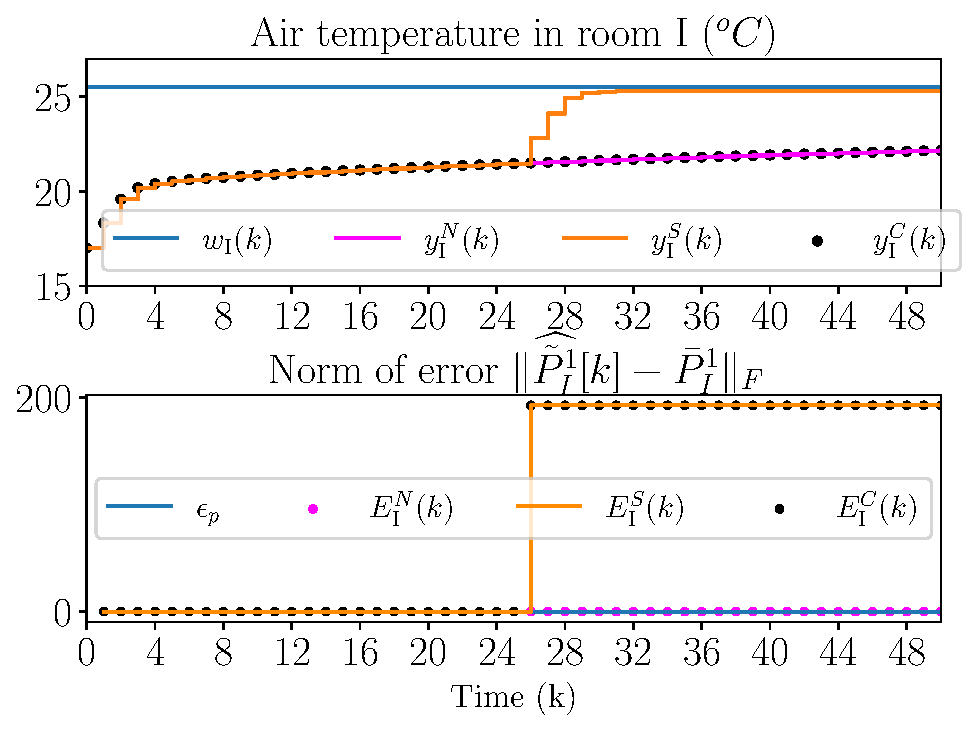
\includegraphics[width=\textwidth]{../img/airtemp_roomI/__ErrorWX_command_normErrH_poster.pdf}
          \caption{\centering Air temperature in room I and the decision variable $E_{I}[k]$ for three scenarios: nominal (N), selfish behavior (S),
            and selfish behavior with correction (C).}\label{fig:response3Scenarios}
        \end{figure}
      \end{minipage}
      \hfill
      \begin{minipage}[c]{26cm}
        \begin{figure}[h]
          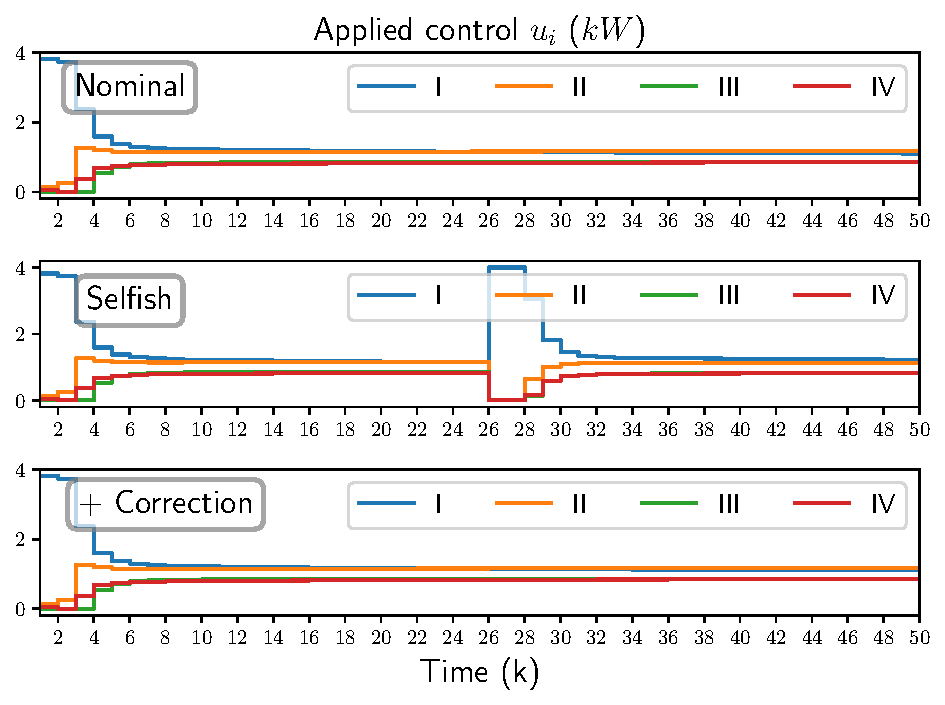
\includegraphics[width=\textwidth]{../img/airtemp_roomI/control_poster.pdf}
          \caption{\centering Control applied in all rooms for the 3 scenarios.}\label{fig:control_3Scenarios}
        \end{figure}
      \end{minipage}
      \hfill
    \end{block}
  \end{textblock}

\end{frame}

\end{document}
